\chapter{Language instantiations}
\label{chp:instantiation}

The model presented in the previous chapter was proposed to be agnostic to
multimedia languages and their syntax. In this section, we discuss the
instantiation of the model entities as first-class citizens and their proposed
syntax in two multimedia languages: NCL (\sect{sec:ncl}) and
HTML (\sect{sec:html}).

\section{NCL instantiation}
\label{sec:ncl}

NCL 3.0 is an XML multimedia language based on the Nested Context Model (NCM)
3.0, a model for hypermedia document specification which allows defining
temporal and spatial relationships among media objects. The current entities of
NCM 3.0 do not focus on representing either modalities different from the
GUI-based ones, or interactions aware of the users who interact with the
application. To overcome these limitations, we first instantiate our entities in
NCM 3.0. \fig{fig:ncm}\footnote{Some NCM entities are omitted from the
discussion here for simplicity (e.g. Descriptor, SwitchPort) or because they
are not used in NCL 3.0 (\textit{e.g.} ConstraintConnector). For a complete
description of NCM, we refer the reader to \cite{soares_nested_2009}}
illustrates the current NCM entities, highlighted in light blue, and our
extensions, highlighted in light green. \appen{annex:schemas} presents XML
schemas, which detail our NCL 3.0 syntax extensions.

The main entities of NCM 3.0 are \textit{Node} and \textit{Link}. We briefly
detail them in what follows.

An NCM 3.0 \textit{Node} is defined by its content, a descriptor, and a list of
anchors.
\textit{Content} is the collection of information of a node. Descriptor defines
properties for how a node should be exhibited, such as position for graphics,
frame rate for video, and volume for audio. The \textit{Anchor}s in the list of
\textit{Anchor}s
can be of two types: \textit{ContentAnchor}, which represents portions of the
content of the node; or \textit{AttributeAnchor}, which represents a property of
the node.
\textit{ContentNode} and \textit{CompositeNode} are specializations of Node and
detail the semantics of Content and \textit{ContentAnchor}. \textit{ContentNode}
has been specialized mainly for 2D audiovisual media modalities, such as
\textit{TextNode}, \textit{ImageNode}, and \textit{VideoNode}.
\textit{ContentAnchor}s of \textit{ContentNode} are spatial or temporal
portions of the corresponding media objects. For instance, the \textit{Content}
of a \textit{VideoNode} may be defined via references to a video file
(\textit{e.g.} file URI) and its temporal anchors by references to
its presentation times.

An NCM \textit{Link} is defined by a \textit{Connector} and a list of
\textit{Bind}s.
\textit{Connectors} define the link semantics, independently of the
participating \textit{Node}s.
More precisely, a \textit{Connector} defines the relation between
\textit{Role}s and not between specific \textit{Node}s. When instantiating a
\textit{Connector}, one \textit{Link} must define the association
(\textit{i.e.}~\textit{Bind}) of each connector \textit{Role} to
a node interface (\textit{ContentAnchor}, \textit{AttributeAnchor} or
\textit{Port}s).

A Role is defined by the attributes: \textit{RoleID}, \textit{EventType},
\textit{minCardinality}, and
\textit{maxCardinality}. The \textit{EventType} refers to a specific event
related to an \textit{Anchor}. NCM 3.0 has three main event types:
\textit{PresentationEvent}, meaning the exhibition of a \textit{ContentAnchor};
\textit{AttributionEvent}, meaning the modification of a node property
(\textit{AttributeAnchor}); and \textit{SelectionEvent}, meaning a mouse click
or key-based event while a specific \textit{ContentAnchor} is occurring. In
particular, the \textit{SelectionEvent} has a key attribute that defines the
key (\textit{e.g.} keyboard or remote control) that triggers the event.

Whereas a connector may represent any kind of relationship between node anchors,
NCL 3.0 defines only the \textit{CausalConnector} relationship.
\textit{CausalConnector} specifies which conditions (\textit{ConditionRoles})
need to be satisfied to trigger actions (\textit{ActionRoles}). A
\textit{ConditionRole} can be a \textit{SimpleCondition} or a
\textit{CompoundCondition}. \textit{SimpleCondition}s act over \textit{Node}s
and may test the occurrence of an event (\textit{e.g.} when the event state
changes to “occurring”). \textit{CompoundCondition}s represent a logical
expression using “and” or “or” operators through \textit{SimpleCondition}s and
\textit{AssessmentSatement}s. An \textit{AssessmentSatement} is used to compare
event attributes. For instance, \textit{SelectionEvent} has a key attribute,
which can be tested in \textit{SimpleCondition} or
\textit{AttributeAssessment}. Finally, \textit{ActionRole} may define changes
in presentation state or properties of \textit{Node}s.

In the remainder of this section (subsections \ref{sec:instantiation:node}
and \ref{sec:instantiations:link}), we present our extensions to NCM and NCL
aiming to address these limitations.

\begin{landscape}
\begin{figure}
	\begin{center}
		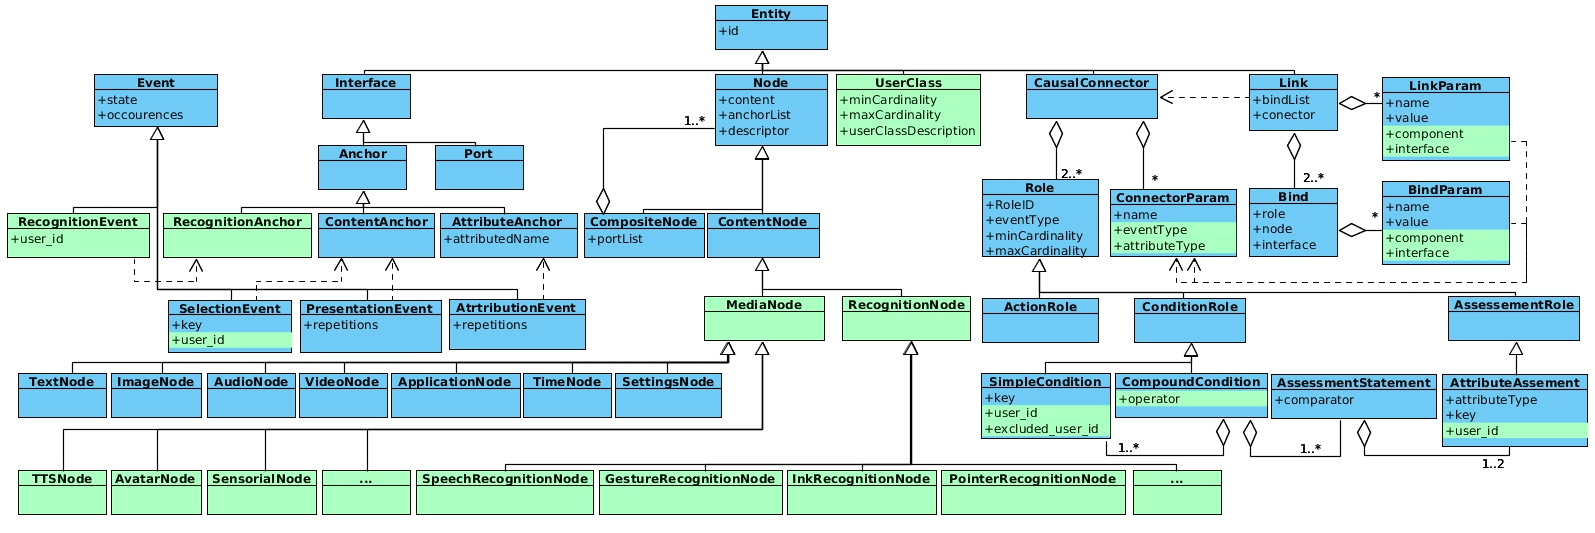
\includegraphics[height=8cm, keepaspectratio]{img/img11.png}
		\caption{NCM 3.0 and proposed extensions.}
		\label{fig:ncm}
	\end{center}
\end{figure}
\end{landscape}

\subsection{Multimodal specializations for Node}
\label{sec:instantiation:node}

To add our \textit{Media} and \textit{Recognizer} entities to NCM 3.0, we
propose multimodal
specializations for Node, named \textit{MediaNode} and \textit{RecognitionNode}.

In a \textit{ContentNode} of NCM 3.0, we group the audiovisual modalities as
specializations of the new \textit{MediaNode} class, which is itself a
specialization of
\textit{ContentNode}. Also, we propose three new \textit{MediaNode}
specializations for
representing output modalities: (1) \textit{TTSNode}, representing a TTS
(Text-To-Speech) content (as described in W3C
SSML~\cite{daniel_c._burnett_speech_2010}, for example), useful
for visually impaired users; (2) \textit{AvatarNode}, representing embodied
conversational agents (\textit{e.g.} described using BML~\cite{vilhjalmsson_behavior_2007}), useful for deaf-,
children- or elderly-oriented interfaces; and (3) \textit{SensorialNode},
representing
sensorial effects (\textit{e.g.} described in MPEG-V SEDL~\cite{iso/iec_iso/iec_2013}), useful for increasing
the QoE~(Quality of Experience)~\cite{ghinea_mulsemedia:_2014} of multimedia presentations. Other
specializations to \textit{MediaNode}
representing other modalities can be seamlessly integrated in the future.

For the representation of input modalities, we propose the new
\textit{RecognitionNode}
as a specialization of \textit{ContentNode}, which can be used in Link
elements. The Content of a \textit{RecognitionNode} is also a collection of
information. Different from the \textit{MediaNode}, however, the information is
expected to be captured, not presented. Some examples of
\textit{RecognitionNode} specializations include: (1)
\textit{SpeechRecognitionNode}, used for speech recognition, such as
recognizing words
and phrases spoken by the user(s); (2) \textit{GestureRecognitionNode}, used
for gesture
recognitions; (3) \textit{InkRecognitionNode}, used for pen writing (“ink”)
recognitions; (4) \textit{PointerRecognitionNode}, used for recognizing
interaction from
a pointer device; and (5) \textit{KeyRecognitionNode}, used for recognizing
interactions
from keyboard devices. Some examples of how the Content of those nodes may be
represented include: W3C SRGS~\cite{andrew_hunt_speech_2004} for \textit{SpeechRecognitionNode}; GDL
(Gesture
Description Language)~\cite{hachaj_semantic_2012} for
\textit{GestureRecognitionNode}; and InkXML~\cite{w3c_ink_2011} for
\textit{InkRecognitionNode}. Also, other specializations to
\textit{RecognitionNode} representing
other input modalities can be seamlessly integrated in the future.

Since \textit{RecognitionNode} is indeed a specialization of
\textit{ContentNode}, it is also
possible to define Anchors in it. A special type of Anchor, the
\textit{RecognitionAnchor}, specifies a portion of the recognition content and
is
associated to a “recognition” event. For instance, a \textit{RecognitionAnchor}
may refer to expected speech tokens defined in a \textit{SpeechRecognitionNode}
or
a “move” or “click” anchor to a \textit{PointerRecognitionNode}. The
“recognition” event indicates that the system has recognized the expected
information defined in a \textit{RecognitionAnchor}. It is important to
highlight that the occurrence of events issued by a \textit{RecognitionNode} is
not intrinsically coupled with \textit{MediaNode} events.

Based on the above extensions to the NCM, we also defined how those changes
can be mapped onto NCL 3.0, the concrete syntax of the model.

NCL 3.0~\cite{abnt_abnt_2016} defines the <media> element for
specifying audiovisual media in a
multimedia document. It has the advantage of being media-type agnostic.
Following the same principle, we propose to use <media> elements to support not
only audiovisual media, but also any type of synthesized description, such as
SSML and SEDL. Therefore, there are no changes in the <media> element.

To allow the integration of \textit{Recognizer} in NCL, we propose a new
element for the
language, named <input>, because NCL 3.0 only considers GUI-based interactions.
Analogous to <media>, <input> defines the \textit{Recognizer} content location
(src),
its properties (<property>), and its anchors (<area>). The src attribute refers
to the Recognizer content, described in languages such as SRGS and GestureML.
To represent that a content was recognized, we define a new event type,
named “recognition” event, which can only be associated to <input> elements.
Similar to other types of events, it introduces reserved words for the start of
the recognition (“onBeginRecognition”) and for its end (“onEndRecognition” or
“onRecognize”).

To illustrate the usage of the these multimodal specializations, we created an
extended version of “Sightseeing of Today”~\cite{fernando_o_2009}, an
interactive non-linear video~\cite{meixner_interactive_2012} about sightseeing
in a city. In its original version, the user interacts
via key/mouse to navigate between videos; in some opportunity time windows, the
user can choose which touristic place the user will be guided next. The choice
is: if the user presses the RED button, the “downtown” video is started; and if
the user presses the GREEN button, then the “beach” video is started. Our
extended version, named “Multimodal Sightseeing of Today”, enables video
navigation also via voice commands.

“Multimodal Sightseeing of Today” uses two multimodal descriptions, an SSML
(\lis{list:ssml}) and an SRGS (\lis{list:srgs}) file, to enable the user to
choose which video to play next.

\lis{list:ncl-sightseeing} shows the code fragment responsible for controlling
the first
navigation. It defines four <media> and one <input> elements. Three <media>
elements (“intro”, “videoDowntown” and “videoBeach”, lines 16-25) define the
introductory video and the two videos available for the user to choose from.
The “intro” video has an anchor (“choice\_moment”) starting at 40 seconds in
the
video. The fourth <media> “audio\_choice” (lines 26) refers to speech synthesis
and the “asr\_places” <input> (lines 27-30) supports voice commands for
navigation control in this first interaction opportunity. This <input> element
defines two anchors mapping onto rules specified in the “places.sgrs” file,
defining the words “downtown” and “beach”.

Regarding the application behavior, it begins by starting the “intro” video
(line 15) and defines three <link> elements. The first link (lines 31-36)
defines that, when the “choice\_moment” anchor is reached, then application
asks
for possible places via voice command. The other two links (lines 37-44) define
that when the user says the name of a recognized place, then the corresponding
video should be started.

\begin{listing}[!ht]
\begin{minted}[linenos,fontsize=\scriptsize,numbersep=1pt,frame=lines,xleftmargin=10pt,framesep=2mm]{xml}
<speak xmlns="http://www.w3.org/2001/10/synthesis">
  <s>Do you want visit the Rio de Janeiro’s downtown or the
  Copacabana beach?</s>
  ...
</speak>
\end{minted}
\caption{downtown\_or\_beach\_audio.ssml.}
\label{list:ssml}
\end{listing}

\begin{listing}[!ht]
\begin{minted}[linenos,fontsize=\scriptsize,numbersep=1pt,frame=lines,xleftmargin=10pt,framesep=2mm]{xml}
<grammar xmlns="http://www.w3.org/2001/06/grammar">
  <rule id="downtown">downtown</rule>
  <rule id="beach">beach</rule>
  ...
</grammar>
\end{minted}
\caption{places.sgrs.}
\label{list:srgs}
\end{listing}

\begin{minted}[linenos,fontsize=\scriptsize,numbersep=1pt,frame=lines,xleftmargin=10pt,framesep=2mm]{xml}
<ncl xmlns="http://www.ncl.org.br/NCL3.0/EDTVProfile">
  <head>
    <connectorBase>
      <causalConnector id="onBeginStart">
        <simpleCondition role="onBegin"/>
        <simpleAction role="start"/>
      </causalConnector>
      <causalConnector id="onRecognizeStart">
        <simpleCondition role="onRecognize"/>
        <simpleAction role="start"/>
      </causalConnector>
    </connectorBase>
  </head>
  <body>
    <port component="intro"/>
    <media id="intro" src="intro.mp4">
      <property name="size" value="100%, 100%"/>
      <area label="choice_moment" begin="40s"/>
    </media>
    <media id="videoDowntown" src="downtown.mp4">
      <property name="size" value="100%, 100%"/>
    </media>
    <media id="videoBeach" src="beach.mp4">
      <property name="size" value="100%, 100%"/>
    </media>
    <media id="audio_choice" src="audio_downtown_or_beach.ssml"/>
    <input id="asr_places" src="places.sgrs">
      <area label="downtown" />
      <area label="beach" />
    </input>
    <link xconnector="onBeginStart">
      <bind role="onBegin" component="intro" interface="choice_moment"/>
      <bind role="start" component="audio_choice"/>
      <bind role="start" component="asr_places" interface="downtown" />
      <bind role="start" component="asr_places" interface="beach"/>
    </link>
    <link xconnector="onRecognizeStart">
      <bind role="onRecognize" component="asr_places" interface="beach"/>
      <bind role="start" component="videoBeach"/>
    </link>
    <link xconnector="onRecognizeStart">
      <bind role="onRecognize" component="asr_places" interface="downtown"/>
      <bind role="start" component="videoDowntown"/>
    </link>
    ...
  </body>
</ncl>
\end{minted}
\begin{listing}[!ht]
\caption{“Multimodal Sightseeing of Today” NCL application.}
\label{list:ncl-sightseeing}
\end{listing}

\subsection{Linking Multiple Modalities and Users}
\label{sec:instantiations:link}

An important feature of MUIs is the combination of interaction modalities.
According to Nigay and Coutaz~\cite{coutaz_four_1995}, this combination can be:
redundant, when only one of the interactions is needed; complementary, when all
interactions are needed; or sequentially complementary, when all interactions
are needed in a specific order. To support these combinations in NCL, authors
may use \textit{CompoundCondition}s with \textit{RecognitionNode}s. Using the
“or” operator, authors can define alternative (redundant) ways in which the user
may interact. Using the “and” operator authors can define complementary
interactions. In addition to the operators already defined by NCM, we include a
new “seq” operator, through which authors can define a required sequence of
interactions. In the “Put-That-There” scenario, for instance, authors must use a
“seq” operator to guarantee that the interactions must occur in the specified
order (first, the “put that”; then, the “logo” selection, etc.).

To enable multiuser features in NCM, we created a new \textit{UserClass} entity.
In NCL 3.03 syntax, we add the <userClass> element defined inside <userBase>, in
the document head (<head> element). It has id, min, max, and
userClassDescription attributes. The userClassDescription is a URL to an
external document describing the UserClass. As previously mentioned,
userClassDescription is tied to how user profiles are specified.

In our proposed instantiation, the system identifies the user and defines their
profiles in RDF (Resource Description Framework)~\cite{w3c_rdf/xml_2014}. Then a \textit{userClassDescription} can use a SPARQL~\cite{w3c_sparql_2008} query to
choose among the users. Each user is a foaf:Person element from the
FOAF~\cite{brickley_foaf_2014} RDF vocabulary, used for user profiles.
Additionally, this foaf:Person may define prf:name elements from
UAProf~\cite{openmobilealliance_wag_2001} RDF vocabulary, used to define device
profiles. The SPARQL query is responsible for selecting which users should be
part of the \textit{UserClass}.

Once having defined a \textit{UserClass}, the developer may define
<simpleCondition> elements using an event attribute named “user\_id”, using the
scheme “user-class-id(user-id)”. For instance, a <simpleCondition> with role and
user\_id attributes with values “onRecognize” and “BoltLikeUser(1)”,
respectively, is trigged only when an interaction is recognized from the first
registered user from the “BoltLikeUser” \textit{UserClass}. Moreover, we define
another optional attribute in <simpleCondition>, called “excluded\_user\_id”. In
this attribute, authors can define the users who are not allowed to trigger a
<simpleCondition>. Such specification of user as parameter is similar to how
Soares~\cite{soares_nested_2009} uses the “key” attribute to define which key
from “selection” events may trigger a link. Indeed, the “user\_id” attribute is
defined for both “selection” and “recognition” events. As in the “key” case, the
“user\_id” attribute may also be tested by developers, in <simpleCondition>
elements.

In our model, the \textit{UserClass} should enable access of runtime properties
related to its users. In the extended NCL, this access occurs though an <media>
element from type “x-ncl-settings” using the scheme: “user-class-id(user-id).
property-name”. For instance, the value “BoltLikeUser(1).canHear” access the
hearing capability of the first registered user from the “BoltLikeUser”
<userClass>.

Finally, it is also interesting to give authors access to the event attributes
through Links. For instance, the author can store the last “user\_id” from a
“recognition” event or the coordinates of a pointer interaction. To do that, we
defined extensions to \textit{ConnectorParam}, \textit{BindParam}, and
\textit{LinkParam}. Besides an arbitrary string value, \textit{ConnectorParam}
can now receive an
\textit{Interface} as well. To define that a \textit{ConnectorParam} should
receive an \textit{Interface}, we propose the
\textit{eventType} and \textit{attributeType} attributes, which are analogous to
those of
\textit{AttributeAssessment}. \textit{BindParam} and \textit{LinkParam} can pass
an Interface as a parameter to Connectors through the component and interface
attributes.

To illustrate the usage of these <link> multimodal and multiuser features,
\appen{annex:scenarios} presents the “Put-That-There” scenario in NCL and its two multiuser versions, namely: “I-Get-That-You-Put-It-There” and
“Anyone-Get-That-Someone-Else-Put-It-There”.


\section{HTML instantiation}
\label{sec:html}

HTML~\cite{w3c_html_2014} is a markup language mainly focused on supporting
text-based interactive content, which has recently included support for audio
and video content (HTML 5.0). Like NCL, HTML does not focus on representing
modalities different from the GUI-based ones, nor about interactions aware of
the users who interact with the application. To overcome these limitations, we
have instantiated our proposed entities in HTML.

At some point, W3C has proposed that HTML should evolve into an XML-based
equivalent, namely XHTML, focusing on XML modularization. The browser vendors,
however, argue that HTML evolution should not follow this path and continue to
use their own markup\footnotemark. Nowadays, when an HTML document, either in
markup or XML syntax, is loaded into a browser engine, it becomes an object
tree following the Document Object Model (DOM) standard~\cite{w3c_dom4_2015}.
The DOM API for HTML, simple called HTML DOM\footnotemark, allows programs
(\textit{e.g.} browsers) and scripts to dynamically access and update the
content, structure, and style of a document, regardless of its syntax
(\textit{e.g.} HTML, XML). \fig{fig:htmldom} illustrates the current HTML DOM
entities\footnotemark, in light blue, and our extensions, in light green. In
particular, the main entities of HTML are \textit{Node} and
\textit{HTMLElement}~\cite{mozilla_dom}.

\footnotetext[2]{\url{https://www.w3.org/TR/html51/introduction.html}}
\footnotetext[3]{\url{https://www.w3schools.com/jsref/dom_obj_document.asp}}
\footnotetext{Some HTML DOM entities are omitted from the discussion here
for simplicity (\textit{e.g.} HTMLBodyElement, HTMLCanvasElement,
HTMLDivElement). For a complete description of HTML, we refer the reader
to~\cite{mozilla_dom}}

\begin{figure}[h]
  \begin{center}
    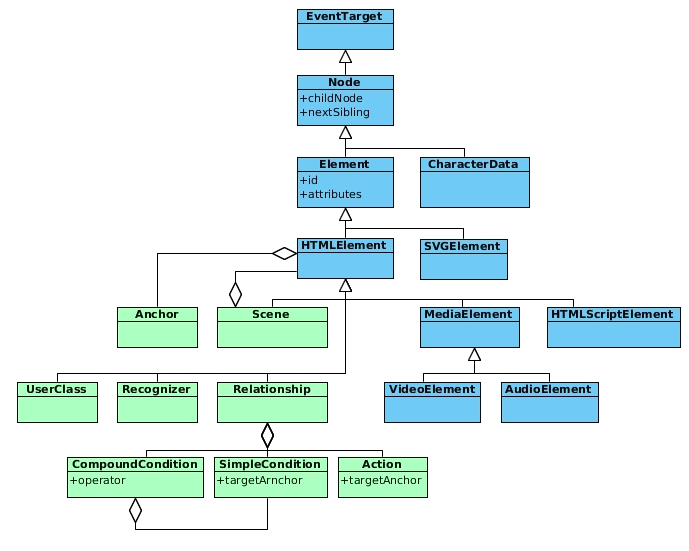
\includegraphics[width=12cm, keepaspectratio]{img/img12.png}
    \captionvspace
    \caption{HTML DOM and proposed extensions}
    \label{fig:htmldom}
    \captionvspace
  \end{center}
\end{figure}

In HTML, everything is a \textit{Node}, including the HTML document itself.
Every \textit{Node} element inherits \textit{EventTarget}, which enables the
scripts elements (HTMLScript) to use the DOM API to register event handlers on
elements in an HTML document. Nested in the HTML document node, there are both
markup elements, namely \textit{Element}, and text only nodes, namely
\textit{CharacterData}. Examples of \textit{Element} are \textit{HTMLElement},
for HTML markup
elements (\textit{e.g.} <div>, <img>, <p>), and
\textit{SVGElement}, for SVG\footnotemark markup elements. Two specializations
of \textit{HTMLElement} are \textit{HTMLScriptElement} and
\textit{MediaElement}. The \textit{HTMLMediaElement}\footnotemark~is the basic
entity for continuous media, such as \textit{HTMLVideoElement} and
\textit{HTMLAudioElement}.

\footnotetext[5]{\url{https://www.w3.org/TR/SVG}}
\footnotetext[6]{\url{https://developer.mozilla.org/en-US/docs/Web/API/HTMLMediaElement}}

We propose to instantiate our entities in the HTML DOM using a browser vendor
standard called \textit{CustomElements}\footnotemark, which provides a
JavaScript API to extend the HTML markup. In other words, it enables developers
to create their own reusable \textit{HTMLElement}s in JavaScript. In our case,
we propose to implement our model entities (\textit{i.e.}~\textit{Media},
\textit{Recognizer}, \textit{Relationship} and \textit{UserClass}) in
JavaScript at runtime. In fact, a similar approach was followed by Soares Neto
\textit{et al.}~\cite{neto_tal_2012}, which at preprocessing time implemented
their template language entities (TAL) using JavaScript.

\footnotetext[7]{\url{https://html.spec.whatwg.org/multipage/custom-elements.html\#custom-elements}}

To implement our \textit{Media} concept, we propose to reuse the existing HTML
audiovisual modalities elements, such as <img>, <audio>, <video>, and to use a
new <mm-media> element to provide synthesized modalities that inherit from
\textit{HTMLElement}. To implement the \textit{Recognizer} concept in HTML, we
propose a new
element <mm-input>. All those elements may use a new <mm-area> to support our
ContentAnchor and RecognitionAnchor elements.

Regarding the \textit{Relationship} entity, we propose the <mm-link>. The
<mm-link> behaves like the NCL <link>, but simplified. All common connectors do
not need to be defined. Simple condition elements may be directly defined by
elements <mm-onBegin>, <mm-onEnd>, and <mm-onRecognize> and action by <mm-start>
and <mm-stop> elements. More than one condition can be grouped in a
<mm-compoundCondtion> element inside a <mm-link>. The <mm-compoundCondition>
should use an operator.

All the proposed elements, may be grouped inside a <mm-scene> element. This
element enables the correct semantics of the <mm-link>. In HTML, <img> or
<video> elements inside the <body> are visible by default. The elements inside
an <mm-scene> are presented only be actions defined in the <mm-link> elements.

To illustrate the usage of this HTML syntax, we implemented the “Multimodal
Sightseeing of Today”. To do that, we use the same SSML (\lis{list:ssml}) and
SRGS (\lis{list:srgs}) multimodal descriptions as in the NCL version.

\lis{list:html-sightseeing} shows the code fragment responsible for controlling
the first navigation. It defines four \textit{Media} and one <mm-input>
element. Three \textit{Media} elements (“intro”, “videoDowntown” and
“videoBeach”, lines 12-19) define the introductory video and the two videos
available for the user to choose from.
The “intro” video has an anchor (“choice\_moment”) starting at 40 seconds in the
video. The fourth <mm-media> “audio\_choice” (lines 20) is speech synthesis and
“asr\_places” <mm-input> (lines 22-26) supports voice commands for navigation
control in this first interaction opportunity. This <mm-input> defines two
anchors mapping onto rules specified in the “places.sgrs” file defining the
words “downtown” and “beach”.

Regarding the application behavior, it begins by starting the “intro” video
(line 8-11) and defines three <mm-link> elements. The first link (lines 27-32)
define that, when the “choice\_moment” anchor is reached, then the application
should ask for possible places via voice command. The other two <mm-links>
(lines 33-40) define that, when the user says the name of a recognized place,
then the corresponding video should be started.

\begin{minted}[linenos,fontsize=\scriptsize,numbersep=1pt,frame=lines,xleftmargin=10pt,framesep=2mm]{xml}
<!DOCTYPE html>
<html>
<head>
  <script src="js/elements/mm.js"></script>
</head>
<body>
  <mm-scene id="scene">
    <mm-link>
      <mm-onBegin interface="scene" />
      <mm-start interface="intro" />
    </mm-link>
    <video id="intro" src="intro.mp4"
      style="position: absolute; height 100%; width: 100%;">
      <mm-area id="choice_moment" begin="40s" />
    </video>
    <video id="videoDowntown" src="downtown.mp4"
      style="position: absolute; height 100%; width: 100%;">
    <video id="videoBeach" src="beach.mp4"
      style="position: absolute; height 100%; width: 100%;">
    <mm-media id="audio_choice"
      src="audio_downtown_or_beach.ssml" />
    <mm-input id="asr_places"
      src="places.sgrs">
      <mm-area label="downtown" />
      <mm-area label="beach" />
    </mm-input>
    <mm-link>
      <mm-onBegin interface="intro.choice_moment" />
      <mm-start interface="audio_choice" />
      <mm-start interface="asr_places.downtown" />
      <mm-start interface="asr_places.beach" />
    </mm-link>
    <mm-link>
      <mm-onRecognize interface="asr_places.beach" />
      <mm-start interface="videoBeach" />
    </mm-link>
    <mm-link>
      <mm-onRecognize interface="asr_places.downtown" />
      <mm-start interface="videoDowntown" />
    </mm-link>
  </mm-scene>
</body>
</html>
\end{minted}
\begin{listing}[!hb]
\caption{“Multimodal Sightseeing of Today” HTML application.}
\label{list:html-sightseeing}
\end{listing}

Finally, we create a new <mm-userClass> with id, min, max, and
\textit{userClassDescription} attributes. The \textit{userClassDescription} is
a URL to a SPARQL
document~\cite{w3c_sparql_2008} defining the required characteristics of the users. Once having
defined an <mm-userClass>, the developer may define <mm-Selection> and
<mm-onRecognize> elements using an event attribute named “user\_id”.